\section{Experiment inventory and main results}
All metrics below are p$K_d$ evaluation results. A missing field is not filled from a neighboring run. Runs with different batch size, seed, stopping rule or input scaling are separate experiment conditions.

\begin{table*}[tb]\centering\small
\caption{Audited Davis experiments. Test metrics are not used here to select a model.}
\label{tab:results}
\begin{tabularx}{\linewidth}{lrrrrrrX}
\toprule Run & Seed & Batch & Epochs (done/requested) & Best epoch & Test MSE & RMSE / CI / $r_m^2$ & Status and evidence \\
\midrule
Primary, raw & 42 & 32 & 112/150 & 91 & .2570 & .5070 / .8790 / .6817 & Manually stopped; corrected evaluation JSON and 112-row history. \\
Fast, raw & 42 & 512 & 182/400 & 142 & .2403 & .4902 / .8840 / .6712 & Early stopped at patience 40; separate run/configuration. \\
Fast, scaled & 42 & 512* & 122/400* & 122 & .2647 & .5145 / .8856 / .5956 & Evaluation JSON + history; full launch metadata unavailable. \\
Retry seed 44 & 44 & 32 & 150/150 & 150 & .4242 & .6513 / .8162 / .4668 & Checkpoint metrics re-evaluated; process status conflict. \\
Retry seed 45 & 45 & 32 & 150/150 & 145 & .4375 & .6614 / .8232 / .4403 & Checkpoint metrics re-evaluated; failure manifest records exit 1. \\
Retry seed 46 & 46 & 32 & 150/150 & 148 & .4013 & .6335 / .8352 / .4925 & Checkpoint metrics re-evaluated; summary/failure conflict. \\
\bottomrule
\end{tabularx}
\end{table*}
\noindent\footnotesize *Scaled-run settings are inherited from experiment documentation and are not fully verified by a run manifest.\normalsize

Figure~\ref{fig:curves} plots training and validation history values directly from the CSVs. The primary curve ends at epoch 112 by manual interruption. The fast unscaled curve ends at epoch 182 after patience-based stopping. The scaled run’s history has 122 rows and ends on its best validation epoch; without final run metadata its stopping cause remains uncertain. The runs have different batch sizes and should not be read as a one-factor comparison.

\begin{figure}[tb]\centering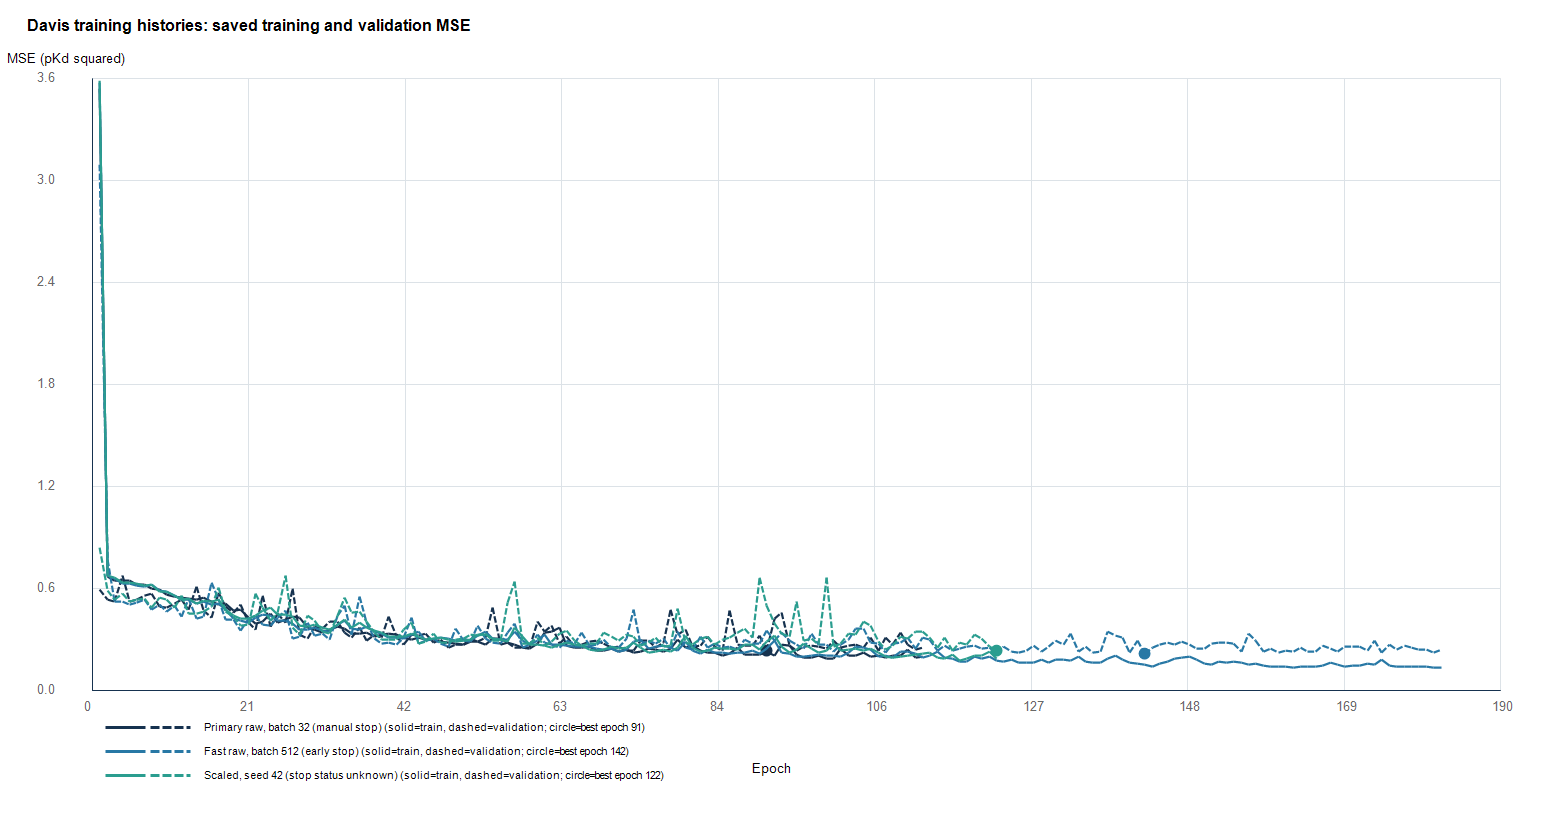
\includegraphics[width=0.97\linewidth]{figures/training_histories.png}\caption{Training and validation MSE from saved histories. Dotted vertical markers identify each recorded best validation epoch; run endpoints differ. Curves are not resampled or extended.}\label{fig:curves}\end{figure}

Figure~\ref{fig:metrics} compares each metric in its own panel because their ranges and interpretation differ. The primary and fast raw runs have similar ranking scores but different error/calibration values; seed 44--46 results are weaker under their batch-32, 150-epoch setup. This is descriptive, not a hyperparameter ranking: the conditions are not controlled across all rows.
\begin{figure}[tb]\centering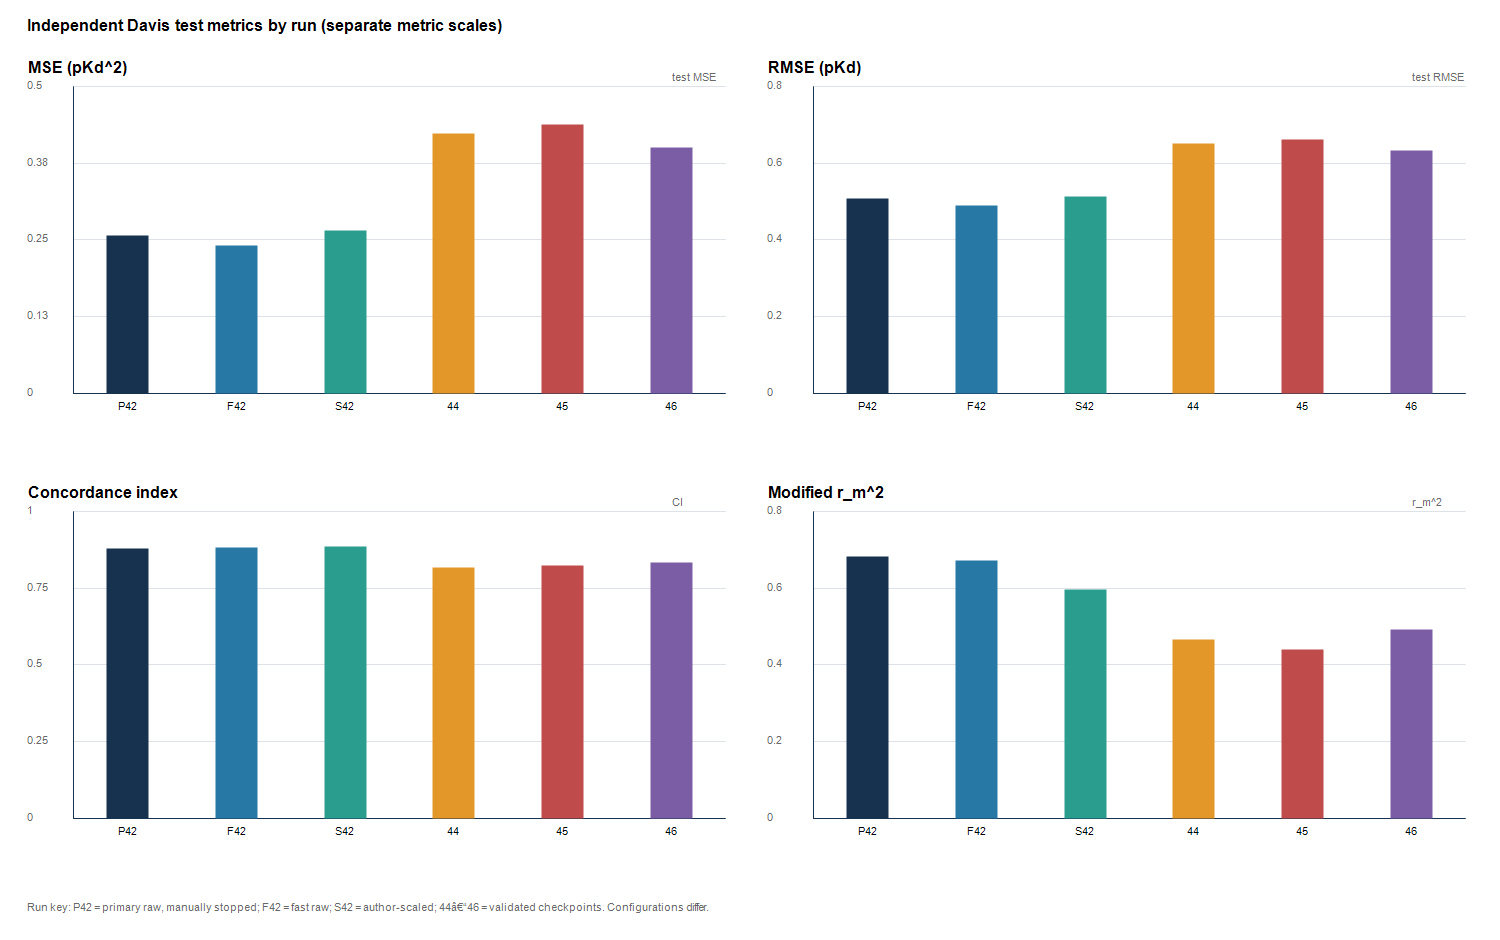
\includegraphics[width=0.97\linewidth]{figures/metric_comparison.png}\caption{Saved test metrics by run, separated by metric. Values are read from the run JSON files; lower is better for MSE/RMSE, higher for CI/$r_m^2$.}\label{fig:metrics}\end{figure}

\section{Feature-scaling experiment}
\textbf{Question.} How do recorded results differ between the raw-feature and author-scaled feature paths? The author transformation is a per-molecule global min--max applied to the full node-feature matrix. A local feature-only audit compared all 68 ligands and 2,180 atoms with the pinned author implementation; it found raw feature values match, while the scaling transform changes their ranges. A separate optional dataset bundle records provenance and hashes.

The two seed-42 results available for a model-level comparison are fast unscaled (batch 512; MSE .2403, RMSE .4902, CI .8840, $r_m^2$ .6712) and fast scaled (evaluation JSON; MSE .2647, RMSE .5145, CI .8856, $r_m^2$ .5956). The scaled run lacks full launch metadata; history lengths and best epochs differ, and the exact commands are unavailable. Figure~\ref{fig:scaling} presents the recorded numbers but cannot isolate scaling as the cause of the differences. No claim that scaling improves or harms predictive performance is justified.
\begin{figure}[tb]\centering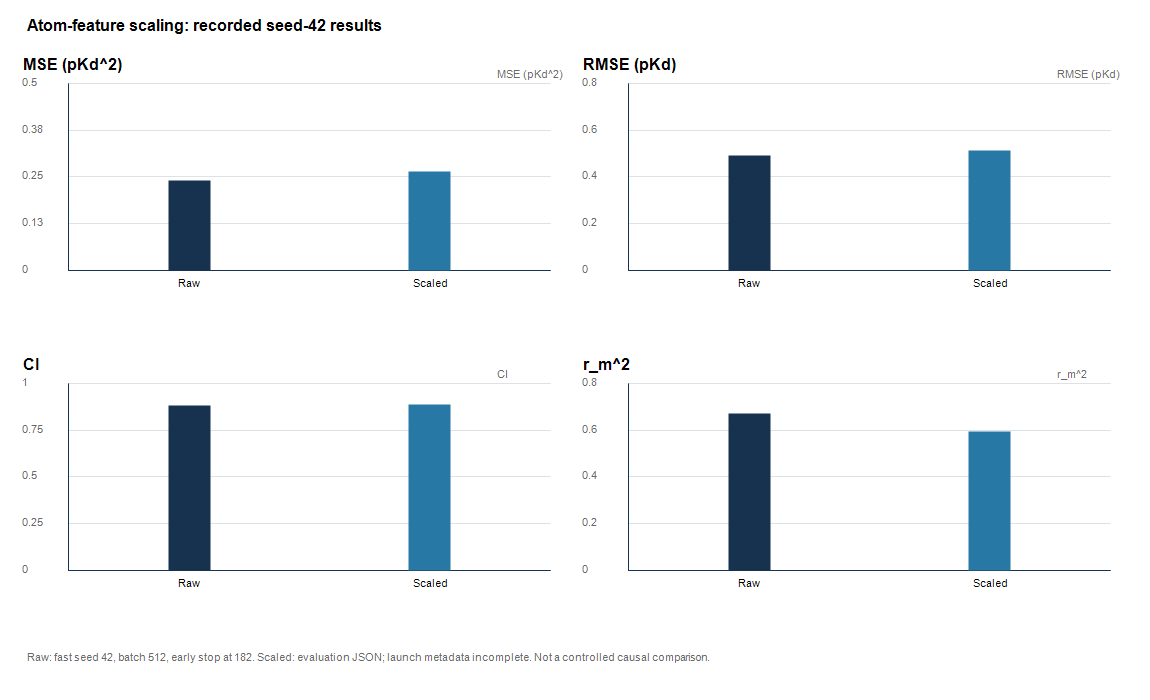
\includegraphics[width=0.87\linewidth]{figures/scaling_comparison.png}\caption{Seed-42 raw versus author-scaled atom-feature results. This is a descriptive comparison with incomplete scaled-run metadata and non-matched stopping histories, not a causal ablation.}\label{fig:scaling}\end{figure}

The additional `scaling_ablation_v1/unscaled/seed_42` directory has a 44-epoch history and checkpoint but no final metrics; it is incomplete and is not included in this plot. Feature-table parity tests and preprocessing checks are evidence of implementation correctness, not evidence of predictive benefit.

\section{Multi-seed checkpoint evaluations}
The validated summary includes seeds 44, 45 and 46. Their three checkpoints each have 150 sequential history rows; best epoch/loss match history and checkpoint metadata. A fresh checkpoint-only evaluation on the current processed test table reproduced all four saved metrics within absolute tolerance $10^{-6}$. Their mean $\pm$ sample standard deviation (ddof=1) is MSE $0.4210\pm0.0183$, RMSE $0.6487\pm0.0141$, CI $0.8248\pm0.0096$, and $r_m^2$ $0.4665\pm0.0261$ (Figure~\ref{fig:seeds}).

This metric validation does not resolve process status. The failure manifest lists exit code 1 for seed 45, despite complete-looking artifacts; older summary files report different states. Seeds 44 and 46 are marked failed in an earlier summary but have no matching entry in the later failure manifest. Thus training artifacts and test-metric reproducibility are supported, while process completion history remains unresolved. The old `multiseed/` set has zero valid runs and empty histories; it is excluded. The summary uses only the identifiable 44--46 checkpoints and is not evidence of a clean successful three-process campaign.
\begin{figure}[tb]\centering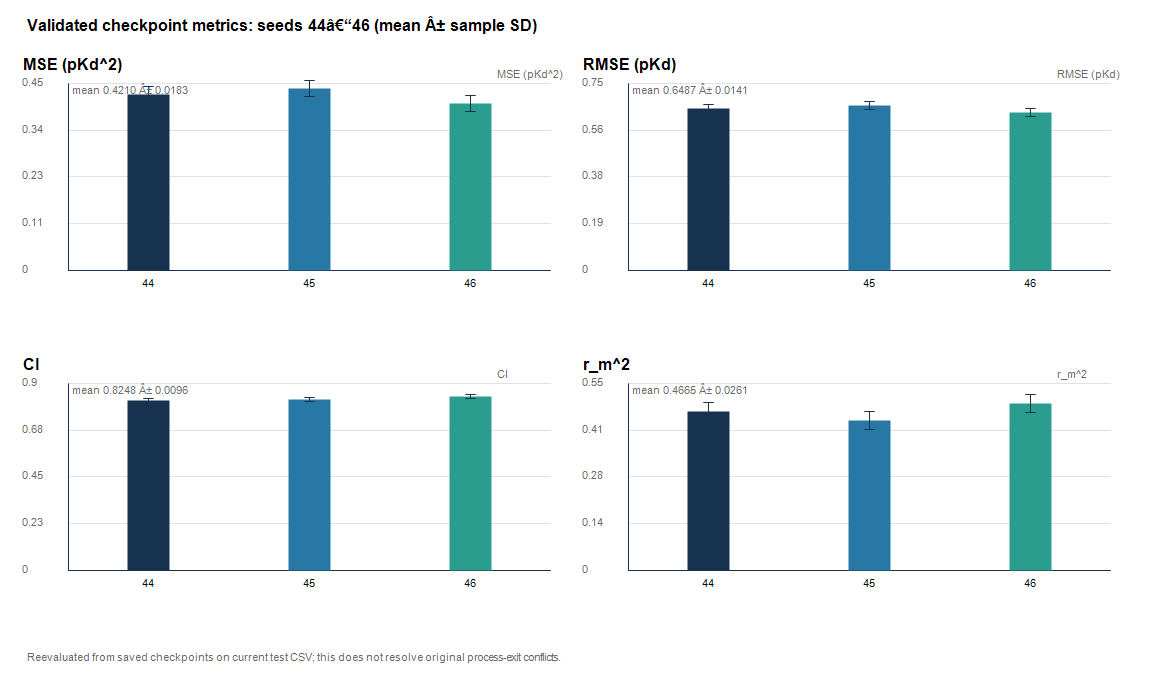
\includegraphics[width=0.88\linewidth]{figures/multiseed_variability.png}\caption{Per-seed metrics for validated checkpoint evaluations (seeds 44--46); markers show the reported mean and whiskers show sample standard deviation. Process-status conflicts remain separate from metric reproduction.}\label{fig:seeds}\end{figure}

\section{Separate protein-graph experiment}
The protein-GNN experiment replaces the main model’s sequence MCNN with a residue graph built from sequence adjacency and a GCN encoder. It retained the drug graph branch and fusion/head concept. Its recorded configuration is seed 42, batch 32, learning rate 0.0005, 50 steps per epoch, 30 requested/completed epochs, patience 10; best validation epoch 29. Test metrics were MSE .6517, RMSE .8073, CI .7597, $r_m^2$ .2090 over 5,010 interactions. This is an exploratory architecture experiment, not a main-MGraphDTA run. A sequence-adjacency graph does not encode 3D contacts or protein geometry; the result cannot establish that graph representations are inherently worse.

\section{Molecular and structural demonstrations}
Figure~\ref{fig:chemistry} shows a representative Davis test molecule using the project’s atom-level Grad-AAM overlay. In the graph model, its atoms are node indices and bonds are edge pairs; the drawing is a two-dimensional rendering of that molecular topology. Color indicates normalized model attribution for the selected prediction, not a physical binding contact.

The repository also contains five independent coordinate-based demonstrations under `results/demos/protein_ligand_interactions/`. The selected examples in Figure~\ref{fig:structures} are deposited X-ray complexes 2HYY (ABL1–imatinib) and 2ITZ (EGFR L858R–gefitinib). Their interaction diagrams summarize geometric screens from deposited coordinates using documented distance/angle criteria; they are demonstrations, not Davis model outputs, and not affinity predictions. The verification notes caution that structures generally lack hydrogens and that geometric screens are not protonation-aware energy calculations.

\begin{figure}[tb]\centering
\begin{subfigure}{0.48\linewidth}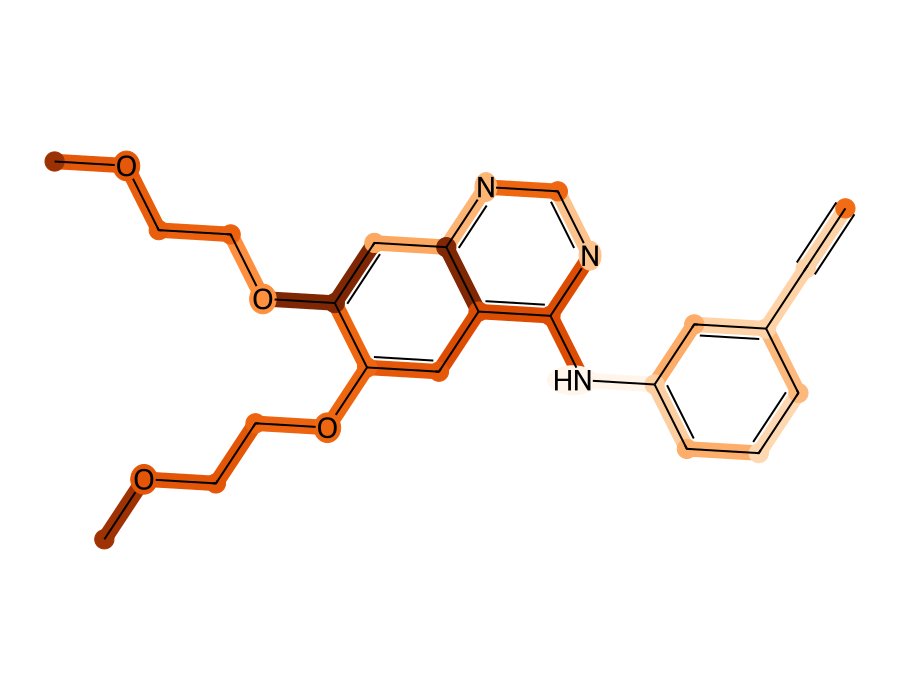
\includegraphics[width=\linewidth]{figures/grad_aam_0.png}\caption{Davis test sample 0 (29 atoms).}\end{subfigure}\hfill
\begin{subfigure}{0.48\linewidth}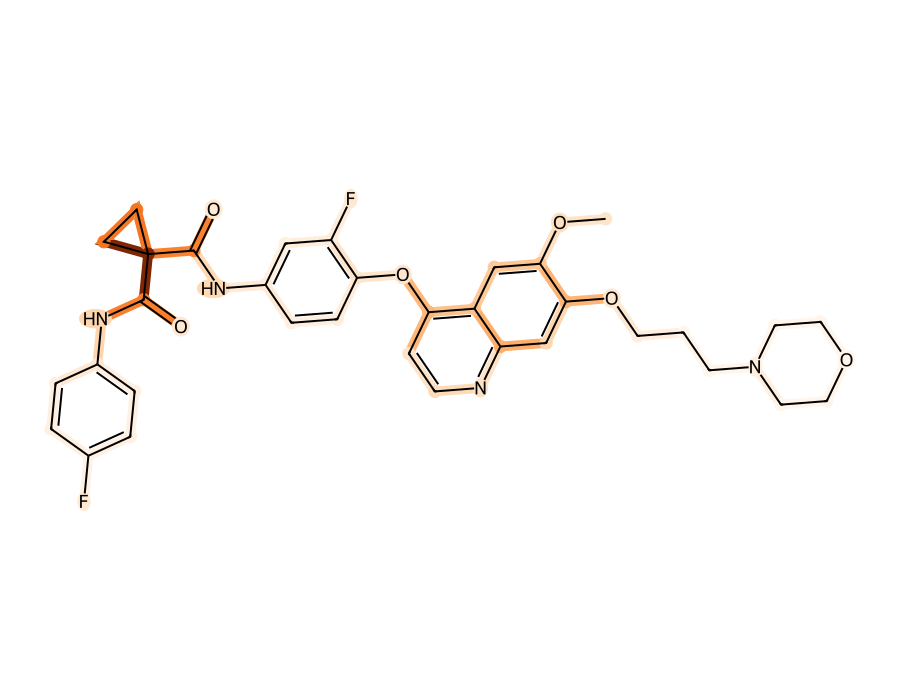
\includegraphics[width=\linewidth]{figures/grad_aam_3.png}\caption{Davis test sample 3 (46 atoms).}\end{subfigure}
\caption{RDKit 2D molecular renderings with Grad-AAM atom importance. Orange intensity represents normalized sensitivity under the implemented method. Neither map establishes a causal biochemical interaction. Sample metadata is retained in the corresponding JSON files.}\label{fig:chemistry}\end{figure}

\begin{figure}[tb]\centering
\begin{subfigure}{0.48\linewidth}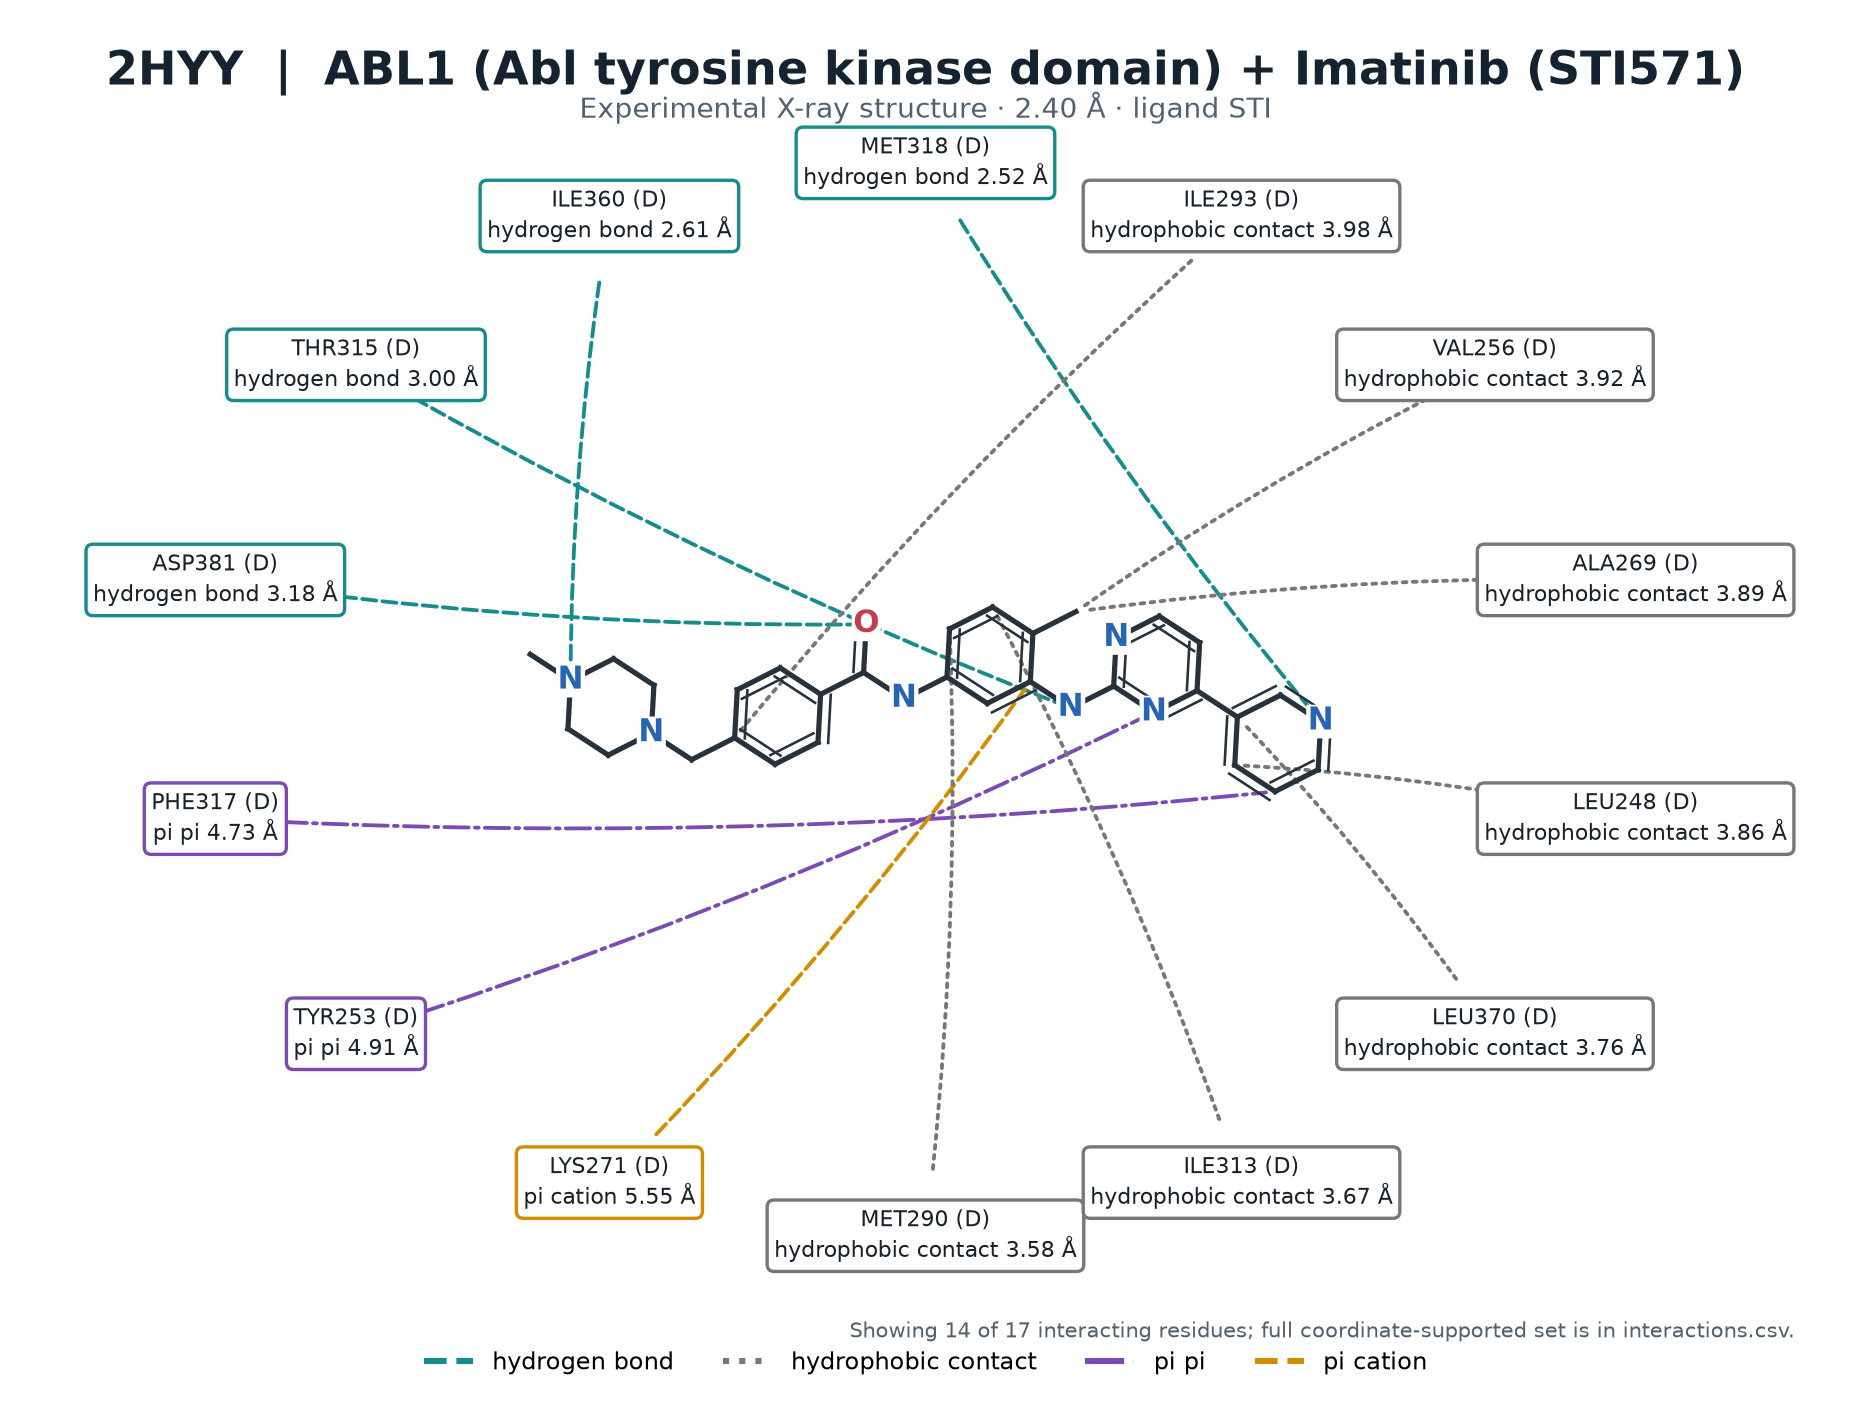
\includegraphics[width=\linewidth]{figures/interaction_2HYY.png}\caption{2HYY: ABL1 and imatinib.}\end{subfigure}\hfill
\begin{subfigure}{0.48\linewidth}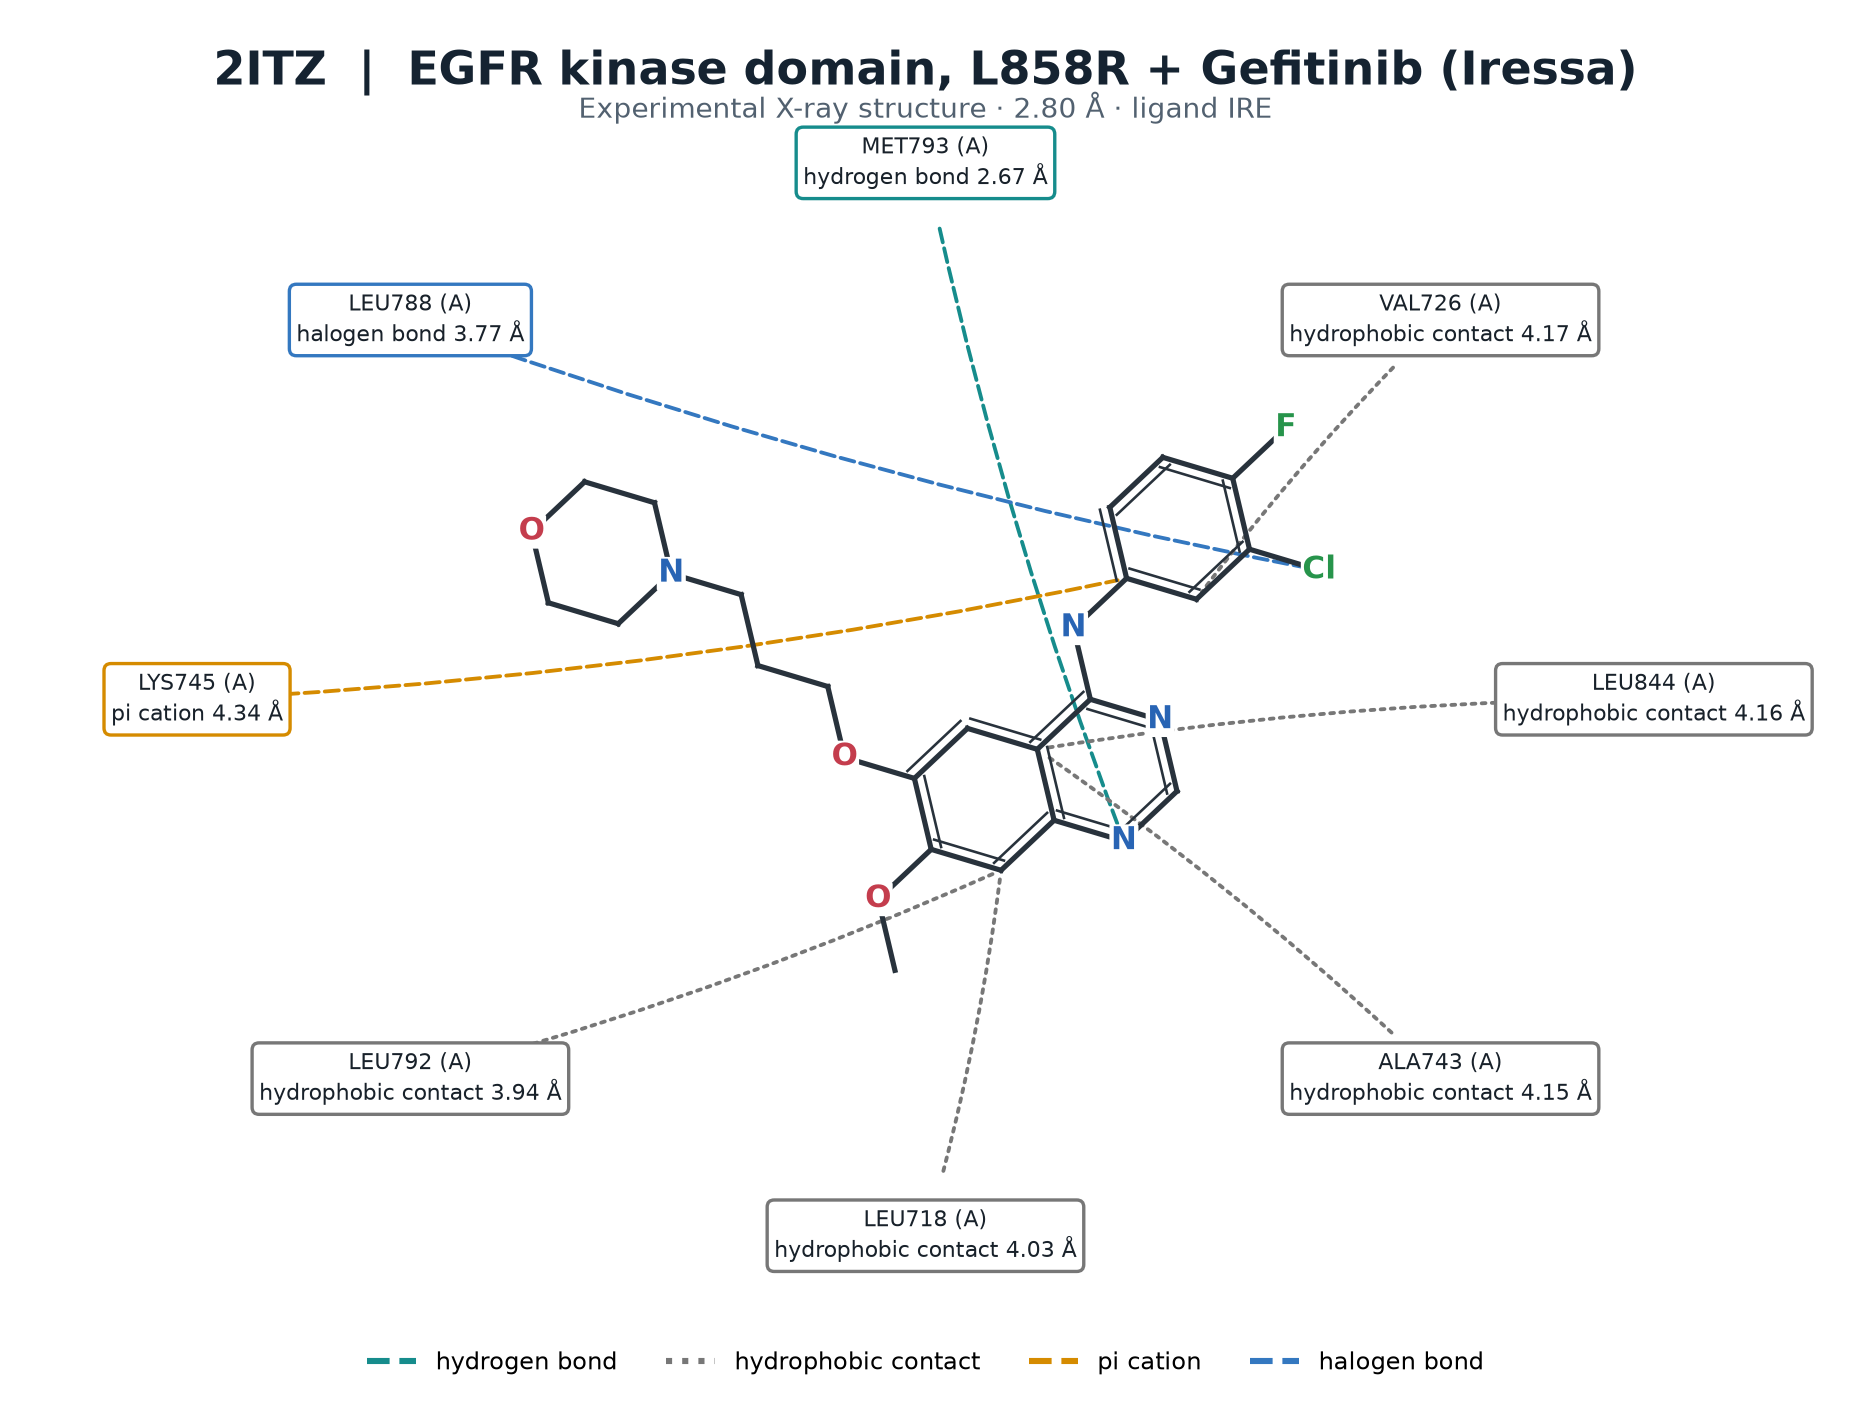
\includegraphics[width=\linewidth]{figures/interaction_2ITZ.png}\caption{2ITZ: EGFR L858R and gefitinib.}\end{subfigure}
\caption{Independent structure-based interaction demonstrations from experimental X-ray coordinates \citep{rcsb2hyy,rcsb2itz}. Lines/contacts are the project's geometric annotations, not interactions predicted by the Davis MGraphDTA model. See each example’s verification note for criteria and limitations.}\label{fig:structures}\end{figure}

